%% ****** Start of file apstemplate.tex ****** %
%%
%%
%%   This file is part of the APS files in the REVTeX 4 distribution.
%%   Version 4.1r of REVTeX, August 2010
%%
%%
%%   Copyright (c) 2001, 2009, 2010 The American Physical Society.
%%
%%   See the REVTeX 4 README file for restrictions and more information.
%%
%
% This is a template for producing manuscripts for use with REVTEX 4.0
% Copy this file to another name and then work on that file.
% That way, you always have this original template file to use.
%
% Group addresses by affiliation; use superscriptaddress for long
% author lists, or if there are many overlapping affiliations.
% For Phys. Rev. appearance, change preprint to twocolumn.
% Choose pra, prb, prc, prd, pre, prl, prstab, prstper, or rmp for journal
%  Add 'draft' option to mark overfull boxes with black boxes
%  Add 'showpacs' option to make PACS codes appear
%  Add 'showkeys' option to make keywords appear
%\documentclass[aps,prl,preprint,groupedaddress]{revtex4-1}
%\documentclass[aps,prl,preprint,superscriptaddress]{revtex4-1}
\documentclass[aps,pra,reprint,superscriptaddress]{revtex4-1}

% You should use BibTeX and apsrev.bst for references
% Choosing a journal automatically selects the correct APS
% BibTeX style file (bst file), so only uncomment the line
% below if necessary.
%\bibliographystyle{apsrev4-1}

\usepackage{graphicx}% Include figure files
\usepackage{dcolumn}% Align table columns on decimal point
\usepackage{clrscode}
\usepackage{bm}% bold math
\usepackage{xcolor}
\usepackage{amsmath}
\usepackage{hyperref}
\usepackage{braket}
\usepackage{bbold}
\usepackage{verbatim}
\usepackage{caption}
\usepackage{subcaption}


\begin{document}

% Use the \preprint command to place your local institutional report
% number in the upper righthand corner of the title page in preprint mode.
% Multiple \preprint commands are allowed.
% Use the 'preprintnumbers' class option to override journal defaults
% to display numbers if necessary
%\preprint{}

%Title of paper
\title{Investigating BEC behavior in the Shake Up Challenge}

% repeat the \author .. \affiliation  etc. as needed
% \email, \thanks, \homepage, \altaffiliation all apply to the current
% author. Explanatory text should go in the []'s, actual e-mail
% address or url should go in the {}'s for \email and \homepage.
% Please use the appropriate macro foreach each type of information

% \affiliation command applies to all authors since the last
% \affiliation command. The \affiliation command should follow the
% other information
% \affiliation can be followed by \email, \homepage, \thanks as well.
\author{Tobias Rasmussen}
\affiliation{Department of Physics and Astronomy, Aarhus University, Ny Munkegade 120, 8000 Aarhus C, Denmark}
\email{201608265@post.au.dk}
%\homepage[]{Your web page}
%\thanks{}
%\altaffiliation{}


%Collaboration name if desired (requires use of superscriptaddress
%option in \documentclass). \noaffiliation is required (may also be
%used with the \author command).
%\collaboration can be followed by \email, \homepage, \thanks as well.
%\collaboration{}
%\noaffiliation

\date{September 18\textsuperscript{th}, 2020}

%\begin{abstract}
% insert abstract here
%{This is a very preliminary document describing the efforts regarding implementation of spintronic systems in the Aarhus University quantum gas microscope.}
%\end{abstract}

% insert suggested PACS numbers in braces on next line
%\pacs{37.25.+k,37.10.Jk, 03.75.Dg}
% insert suggested keywords - APS authors don't need to do this
%\keywords{}

%\maketitle must follow title, authors, abstract, \pacs, and \keywords
\maketitle

% body of paper here - Use proper section commands

\section{Introduction}
%Here, you should write an introduction that describes what specific problems you explored. Your introduction should also describe how the document is structured (e.g. ``Section \ref{sec:back} describes how I invented underwater basket weaving for Bose-Einstein condensates...''). You should also briefly describe the main results, but keep this to a sentence or two. The rest of the report should elaborate on those results and the methods you used to find them.
In the Shake Up challenge, one works with a state confined in a trapping potential. The state describes either a single particle or a Bose Einstein Condensate (BEC) state of matter and starts in the ground state of the given potential. The goal is now to translate the potential in such a way that the state is completely excited from its ground state to its first excited state. The potential is moved using a control function $u(t)$, which in this challenge can be either an analytical function or created by dragging a path on a graphical interface in the program Quantum Composer. This is also the software on which this problem is simulated. One uses the fidelity $F = | \langle \phi | \psi \rangle |^2$ to calculate how much of the state $\ket{\psi}$ 'is in' the desired state $\ket{\phi}$ and so as a measure for how well a given control function performed.\\

Furthermore, the self picked goal of the workshop was to explore the different dynamics that arise when simulating the BEC compared to a single particle, how these dynamics depend on the factor $\beta$ from \eqref{eq:Hbec} and finally how $\beta$ affects the Quantum Speed Limit (QSL).\\

Section \ref{sec:results} contains the results of the report and is split into 2 parts. Section \ref{subsec:obs} shows the results of simulating BECs under different initial conditions, while section \ref{subsec:strats} explains the strategies used to reach those results. The results are then discussed in section \ref{sec:disc}. 

In section \ref{sec:conclusion} it is concluded that the nonlinear term for the BEC drastically changes the behavior of the state compared to the single particle state for values of $\beta$. This new behavior could in some cases improve the reachable fidelity compared to a single particle by up to $50\%$. It was also found that the value of $\beta$ affects the QSL of BECs. This section also sums up the conclusions about the different approaches to creating a control function that were used in this project.

\section{\label{sec:back}Background}
%Here, you can describe the background of your problem. What motivated you to explore this particular problem? Describe your general strategy. What do we need to know to understand your results?
The Hamiltonian describing a single particle in a trapped, controlled potential takes the form:
\begin{equation}
	H(x,t) = \frac{p^2}{2m} + V(x,u(t))
\end{equation}
where $p$ is the momentum operator and $m$ is the particle mass. Likewise, the Hamiltonian of a BEC can be approximated to obey the Gross-Pitaevskii equation
\begin{equation}
	H_{BEC} = \frac{p^2}{2m} + V(x,u(t)) + \beta |\psi(x,t)|^2
	\label{eq:Hbec}
\end{equation}
which contains a nonlinear term with front factor $\beta$ compared to the Hamiltonian for a single particle. This term represents the inter atomic interaction that takes place in a BEC. We get from the Gross-Pitaevskii equation that $\beta = 4\pi\hbar^2 a_s / m$ with $a_s$ being the s-wave scattering length for 2 interacting bosons and $m$ being the mass of the boson.

The problem was explored by adjusting $\beta$, the control final time $T$, the control function $u(t)$ as well as working with both an anharmonic and a harmonic potential.

It is possible to optimize a control function to, in many cases, reach even higher fidelity than this initial function. In this problem the optimization algorithm $\proc{Grape}$ is used. $\proc{Grape}$ takes in the control function (a "seed"), and calculates the gradient of $F$ with respect to each point of the control function on the discrete time scale $\vec{\nabla}_{\vec{u}}F(\vec{u})$, such that $\vec{u} = (u(t_0), u(t_1) ... \,, u(T))$. When this calculation is done, $\proc{Grape}$ takes a step of size $\alpha_k$ such that the new discretized control function becomes
\begin{equation}
	\vec{u}_{k+1} = \vec{u}_{k} + \alpha_k \vec{\nabla}_{\vec{u}}F(\vec{u}_k)
\end{equation}
where $F(\vec{u}_{k+1}) \geq F(\vec{u}_{k})$.

This process is continued until some convergence criterium is fulfilled, e.g. a target threshold $F(\vec{u}_{k}) \geq F_{target}$ or a maximum number of iterations $k \leq N$.


\section{\label{sec:results}Results}
%This should be the bulk of your report. Describe your results. Any details (not included in the background) that are necessary to understand what you did should be here.

%You can include citations with the \verb+\cite{}+ command. You will need a \verb+.bib+ file like the one included with this template. See the bibliography file for information on how to cite an article \cite{Schmiedmayer2014}, a thesis \cite{HenrikThesis}, or a book \cite{PethickSmith}. If you do not include any citations, comment the \verb+\bibliography{}+ command below.

% Potentials used
Two different potentials were used during this project: One harmonic and one anharmonic. They can both be expressed
\begin{equation}
	V(x, u(t)) = \frac{a^2}{2}(x-u(t))^2 + \frac{b^4}{2}(x-u(t))^4
	\label{eq:potential}
\end{equation}
where $a = 10$ in both cases and $b=4$ in the anharmonic case and $0$ in the harmonic case. $u(t)$ is the control function which translates the potential as a function of time. These potentials will simply be referred to as 'the' (an)harmonic potenial.

% I use $\proc{Grape}$ from flow files
Whenever optimization of control functions was done, it was using the $\proc{Grape}$ routine with the iteration cap set to $N=50$ and a target fidelity $F_{target} = 0.99$. 


\subsection{\label{subsec:obs}Oberservations}
% Single particle 
Single particles are simple to control. In the anharmonic potential case one can write up many simple control functions which are all able to reach $F\approx0.99$ after at most 25 iterations of $\proc{Grape}$. This is not the case in the harmonic potential since the state is easily excited beyond the desired state due to the same sized energy spacing of a harmonic potential. \\

% BEC in anharmonic
Through simulations it seems that BECs have very different dynamics compared to single particles. Without using $\proc{Grape}$, one can study how the similarity between single particles and BECs change depending on the value of $\beta$. Keeping the control function the same, we find that what was a good solution for a single particle reaches a lower and lower fidelity as we change $\beta$ away from 0, but that it also reaches revivals with a higher fidelity compared to neighboring values. This behavior is shown in figure \ref{fig:beta}.\\


\begin{figure}[h]
	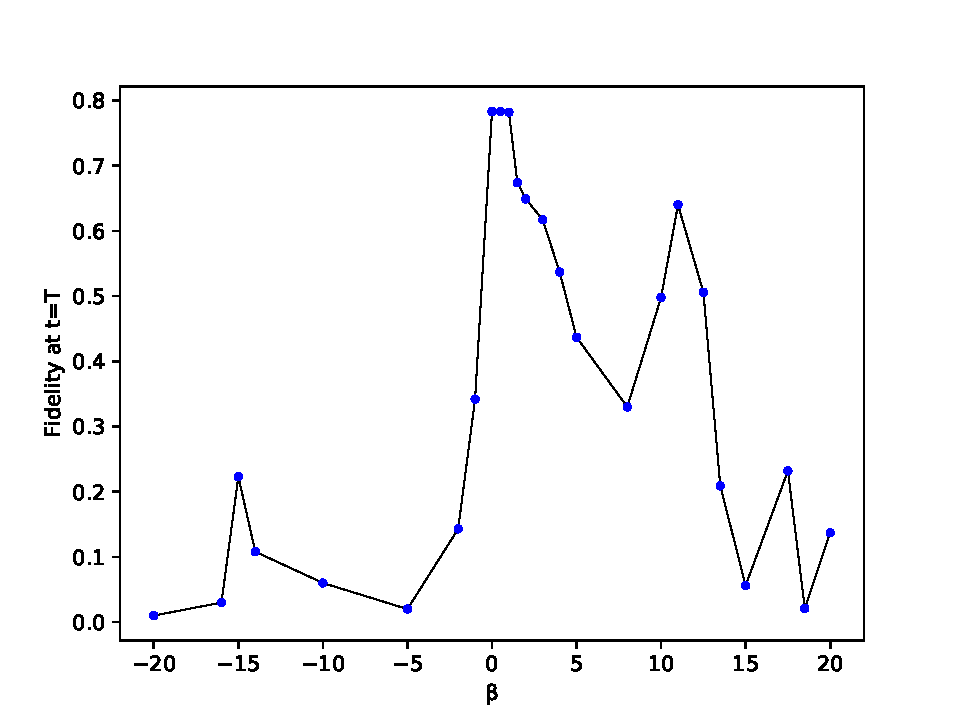
\includegraphics[width=\columnwidth]{graphics/beta.pdf}
	\caption{Fidelity at $t=T$ for different values of $\beta$ with no optimization in the anharmonic potential. The control function was $0.12\cdot\sin(0.86\cdot \omega_{01} t)$ with $T = 3.49$. The constant $\omega_{01}$ is the energy frequency between the ground state and first excited state in this potential.}
	\label{fig:beta}
\end{figure}

\begin{figure}[h]
	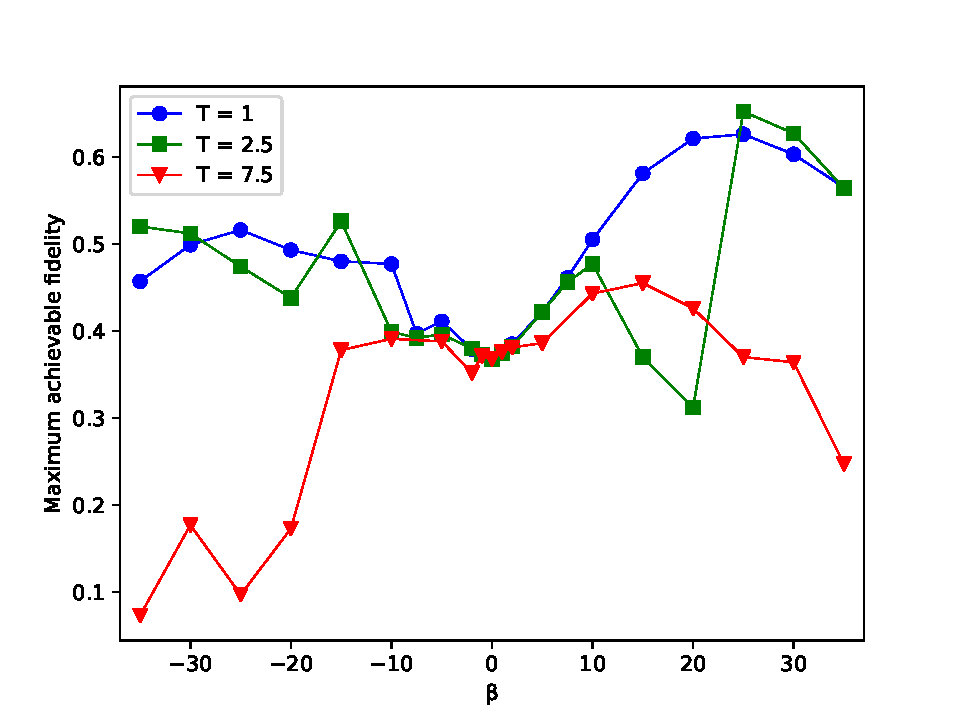
\includegraphics[width=\columnwidth]{graphics/betaTHO.pdf}
	\caption{The result of varying $\beta$ and $T$ for a BEC in the harmonic potential. As it can be seen, there exists 'resonant' combinations where it is possible to achieve above $50\%$ higher fidelity compared to a single particle (at $\beta=0$), but many also combinations that are on par with or worse than a single particle.}
	\label{fig:HO}
\end{figure}

% For large T we observe different behavior for BECs and SPs
As it can be seen in figure \ref{fig:beta}, the value of $\beta$ significantly changes the behavior of the system. When studying BECs in the anharmonic potential, it was found that for small $\beta<5$ it was possible to optimize the state to reach the same high fidelity as for the single particle case. For larger values of $\beta$, it was observed that the final fidelity converged on increasingly smaller values. The fidelity could be improved by raising/lowering the final time $T$, but for large $\beta > 25$ the maximum reachable fidelity with $\proc{Grape}$ decreases to below $0.99$. So obviously there exists some relationship between $\beta$ and $T$ where some combinations result in high fidelity while others do not. This could also explain why some values of $\beta$ in figure \ref{fig:beta} increase the fidelity in a small region (e.g. around $\beta=10$) as if there is some kind of resonance. \\

% BEC in harmonic
The nonlinear interaction term of the BEC Hamiltonian also had the positive effect when handling BECs in the harmonic potential case. Here, this term caused a greater final fidelity for some values of beta than in the single particle case, where it was difficult to reach fidelities as high as $0.4$. This is shown in figure \ref{fig:HO}.\\


%QSL
Studying the Quantum Speed Limit for this problem yields the results shown on figure \ref{fig:QSL}. The figure shows how different values of $\beta$ impacts the QSL for BECs in the anharmonic potential. As it can be seen, $\beta$ values away from 0 raise the speed limit increasingly the further away from 0 they are. \\

\begin{figure}[h]
	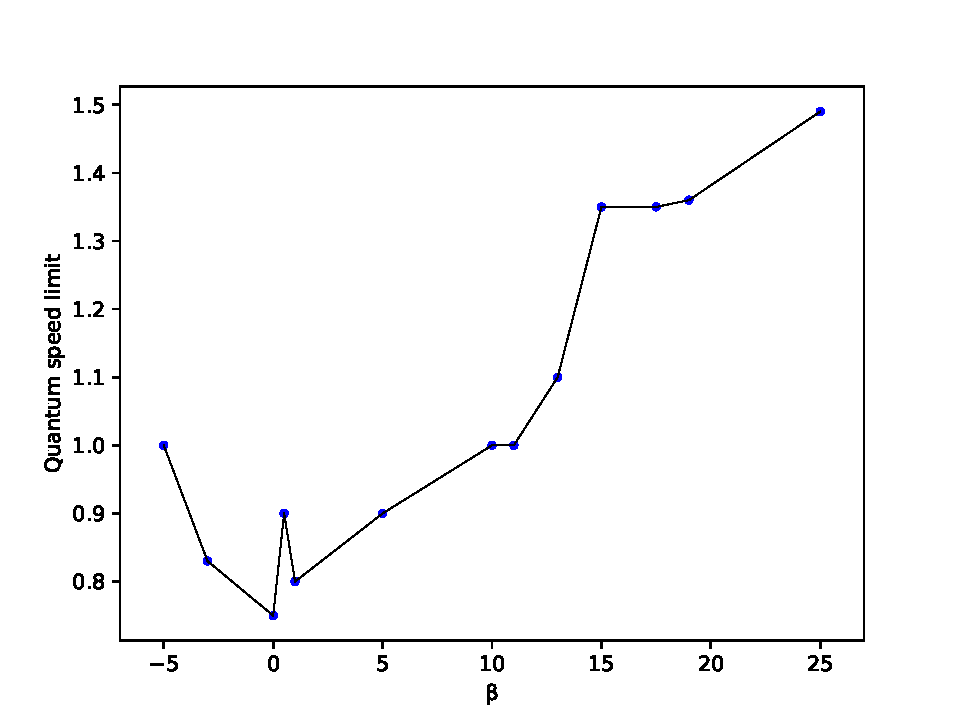
\includegraphics[width=\columnwidth]{graphics/QSL.pdf}
	\caption{The estimated Quantum Speed Limit for a BEC in the anharmonic potential as a function of $\beta$. The behavior of the BEC at $\beta=0$ is the same as for a single particle. Notice how the QSL is doubled compared to a single particle when $\beta=25$. It has not been possible to reach the required fidelity for any $\beta < 5$.}
	\label{fig:QSL}
\end{figure}

It is now clear after having explored the behavior of BECs in different numerical setups that the behavior the BECs are not symmetric with respect to $\beta$. This is not unexpected, since the sign of $\beta$ constitutes whether the atom-atom interaction happening inside the BEC is repulsive($\beta>0$) or attractive ($\beta<0$) and so it would not be unjustified to say that the sign of $\beta$ describe entirely different species of bosons. 

\subsection{\label{subsec:strats}Strategies}
% Function vs graph approach
Throughout working with this project, there has been two ways to determine the control function $u(t)$ in Composer: Either it is determined by an analytical expression (using the Scalar expression node) or it is made by dragging the desired 'path' of displacement on a graph (using the Control node). These different nodes are shown in figure \ref{fig:Controls}. One can use both of these approaches when working with Quantum Control and they both have their advantages and disadvantages. \\

\begin{figure}[h]
	\begin{subfigure}[b]{0.4\columnwidth}
		\centering
		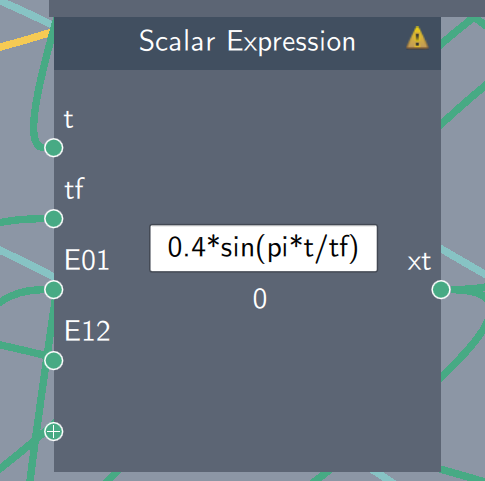
\includegraphics[width=\columnwidth]{graphics/ScalarExpressionNode.png}
		\caption{Scalar expression node}
	\end{subfigure}
	\hfill
	\begin{subfigure}[b]{0.45\columnwidth}
		\centering
		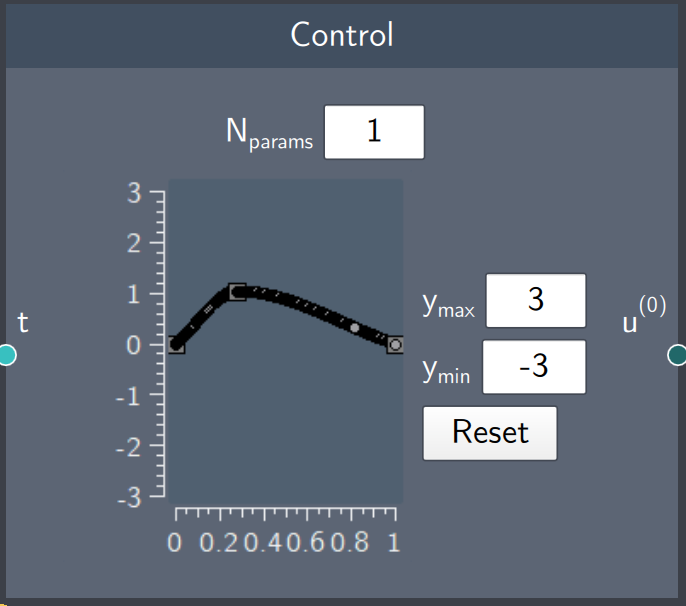
\includegraphics[width=\columnwidth]{graphics/ControlNode.png}
		\caption{Control graph node}
	\end{subfigure}
	\caption{Both nodes used for making a control function in Quantum Composer. The analytical function method (a) can take a number of input constants like final time $tf = T$, energy spacing between different states $(E01 = E_1 - E_0)$ and variables such as time $t$. The graph method (b) always scales the first axis such that the first point on the graph is at $t=t_0$ and the final point is at $t=T$.}
	\label{fig:Controls}
\end{figure}

% About function approach
Using an analytical expression as a control function, one gets the possibility of tweaking initial parameters to great accuracy such that the seed $\proc{Grape}$ gets already has a high fidelity. It is preferable to the graph approach in cases where a desired oscillation frequency is wanted e.g. the function $A\sin(E_{01}*t)$. These kind of functions are difficult to mimic in the graph approach. When working with expressions independent of the final time $T$, adjusting this parameter translates into cutting the graph at different times. This is useful when exploring different functions and one finds that higher fidelity takes place at a different time than one currently works with. This method is shown in figure \ref{fig:funcAppr}. \\
\begin{figure}
	\def\svgwidth{\columnwidth}
	\input{graphics/functionAppr.pdf_tex}
	\caption{This figure shows how using an analytical control function can be used to reach a higher fidelity seed by altering the final time $T$. In this example we use the control function shown in red and the final time $T_1$. Evolving the system for a shorter(longer) time yields a higher fidelity though, and we can reach these fidelities by replacing the final time with $T_2$ ($T_3$). This method only works if the control function is independent of the final time.}
	\label{fig:funcAppr}
\end{figure}

% About graph approach
The Control graph node makes it possible to build up the control function as a series of steps. Here one can move one point on the graph and watch how the state evolves until that point, making it possible to optimize each step before going further. Since the graph node always spans the entire time interval $\{t_0,T\}$, this makes using the node useful when wanting to stretch or contract the entire function as shown on figure \ref{fig:graphAppr}. As demonstrated with the BEC in a harmonic potential in figure \ref{fig:HO}, there exists a complex relationship between $\beta$ and $T$ and so being able to keep the control function the same but altering the total time is a beneficial tool to use.\\

\begin{figure}
	\def\svgwidth{\columnwidth}
	\input{graphics/graphAppr.pdf_tex}
	\caption{A visualization of one method that can be used to optimize fidelity when working with the graph node. If one tries to change the final time $T$ the resulting control function will be squeezed or stretched as a result. Altering the final time can be beneficial given the complex relationship between $\beta$ and $T$, but also as a tool to regulate the speed at which the potential moves. Using this approach also has the practical advantage that we can draw the graph such that $u(T)=0$ and so no matter the final time, the potential will always end up where it started. This is to be compared to the approach shown in figure \ref{fig:funcAppr} where this is not always the case and the state would need to be transported back.}
	\label{fig:graphAppr}
\end{figure}

When calculating the maximum reachable fidelity for some combination of $\beta$ and $T$ in the harmonic potential, the graph control node was used to create for $\proc{Grape}$. The overall strategy using this tool involved moving points on the graph into certain shapes and looking at how the initial (i.e. no $\proc{Grape}$) fidelity looked. I particularly liked the semi-circle shape of a $\sin(\pi t/T)$ function where the amplitude was varied. Another particular shape used was moving a single point around $0.1T$ or $0.9T$ to create a function which had a fast(slow) buildup to a maximum and then a slow(fast) return to the initial position. This nudge-like shape is shown on figure \ref{fig:Controls} (b).

Both these strategies worked well and provided nice seeds for $\proc{Grape}$ to optimize on. Despite some cases where the fidelity changes significantly from small variations of $\beta$, the overall rule seems to be that something that works well for one value of $\beta$ will work okay for nearby $\beta$ and so this was also used to find a good seed when $\beta$ was larger than $10$, since above this limit the system seemed alot more sensitive to the initial control function with respect to reaching the highest possible fidelity for that particular combination of $\beta$ and $T$. \\

Measuring the Quantum Speed Limit for the anharmonic potential involved a combination of 2 strategies: The self-dubbed "up-to-down" and "down-to-up" approaches. \\

The "up-to-down" strategy involved starting with a final time $T_{up}$ which was estimated to lie within the QSL for the value of $\beta$ being measured, $T_{up} > QSL(\beta)$. If this assumption was correct then one should be able to find at least one seed which was optimizable to $F\approx 0.99$. If this was not the case then the final time was raised again and the approach restarted. Assuming that a sufficiently good seed was found for $T_{up}$, the next step is to gradually lower $T$ in small steps, at each step ensuring that $\proc{Grape}$ is still able to optimize the fidelity to $0.99$. If $T$ is lowered such that the seed can no longer reach $0.99$ through $\proc{Grape}$, then small adjustments can be made to see if the seed can be fixed. This was my approach for most of the data seen on figure \ref{fig:QSL}.\\

The "down-to-up" approach works in a different manner, namely that we choose a low $T$ we suspect(guess) to be around/lower than the QSL for this problem. Then we try some different candidates for the control function for this problem and keep the most promising one (measured on reachable fidelity using $\proc{Grape}$). Keeping the current $T$, we can try different small modifications to the control function in an attempt to improve the fidelity further. Should it after these modifications still not be possible to reach $0.99$ fidelity, the next step is to raise $T$ by a small amount and repeat this process of modification again. These final 2 steps are then repeated until $F~0.99$ is reached where the current $T$ is then the estimate of the QSL. 

\section{\label{sec:disc}Discussion}
As explained in section \ref{subsec:strats}, the Quantum Composer software in this workshop allows for 2 different ways to construct control functions. While both methods have been used to explore the behavior of BECs subject to a controlled potential, the files only allow optimization of control functions made using the graph method. 

While the graph method has its advantages as discussed above, the analytical function approach likewise has advantages that could be combined with $\proc{Grape}$. Having multiple approaches to the optimization problem would most likely be beneficial both from a perspective of understanding and from the perspective of being able to fine tune parameters for generating good seeds.\\

From what has been observed partially during exploring the dynamics of BECs and partially while gathering data for figure \ref{fig:HO} and the QSL in figure \ref{fig:QSL}, it is safe to say that when working with high values of $|\beta|$, the behavior of the system becomes difficult to predict. As final time goes up this only becomes more apparent, which was the conclusion that was reached after optimizing BECs in the harmonic potential. 

This raises a (probably realistic)concern that the data shown in those 2 figures have been very sensitive to the initial conditions (i.e. the seed) and that other values could have been reached given more time to try different control functions. This is of course one of the problems with optimizing complex problems in the first place: They can be incredibly sensitive to initial conditions and while finding a local minimum is not a problem, finding the global one is a (very) difficult one.\\

Throughout both the exploration and data collection parts of this workshop, the control functions that have been used have for the most part been simple harmonic functions like $A\sin(\pi t/T)$ or other simple approaches such as the function seen in figure \ref{fig:Controls} b. 

However, what has also become apparent while working with $\proc{Grape}$ is that it usually introduces(after a number of iterations) rapidly oscillating behavior on parts of the graph. It is understood that this is most likely due to the way $\proc{Grape}$ optimizes control functions, but it also shows that more complex control functions are not necessarily bad and can actually in some cases reach much higher fidelity than their 'simpler' counterparts. 

\section{\label{sec:conclusion}Conclusion}
%This section should briefly conclude by describing what you did, your main results, and what you would do if you had time to explore further.

%I have tested the whole realm of quantum mechanics, by inserting random, but nice, numbers into Composer. The results of these high quality borderline genius simulations, was a complete lack of actual physics in the composer engine. Fidelities higher than 100percent is always expected with my skillful shaking of any potential, this is achieved in timescale smaller than my consentration at a kvant II lecture.

%All in all great success!
It has been demonstrated that the behavior of BECs are sensitive to the parameters $\beta$ and $T$. As it has been shown in figure \ref{fig:HO}, this changed behavior compared to a single particle can be beneficial and capable of reaching higher fidelity than is otherwise possible. On the other hand it is also apparent that $\beta$ introduces an unpredictability into the system, where solutions that work well for one value do not work at all for another value, even for nearby values. It has also been shown that the $\beta$ term in \eqref{eq:Hbec} increases the QSL up to a estimated value of 2 times that of a single particle for the case $\beta=25$.

Some strategies involving choosing a control function have also been explored. The differences, advantages and disadvantages of using either an analytical function node or a graph node to determine the control function have been discussed. This includes how varying $T$ affects the control function, as has been illustrated on figures \ref{fig:funcAppr} and \ref{fig:graphAppr}. Finally, 2 concrete strategies for determining the QSL in this problem have been explained, both using the graph node to create a control function. 
% Create the reference section using BibTeX:
% comment the line below if you do not have a bibliography
%\bibliography{thebibliography}

\end{document}